% !TeX root = ../main.tex

\begin{figure}[htbp]
  \centering
  
\includegraphics[trim=200 200 200 200, clip, width=0.45\textwidth]{figures/surf-side.png}
  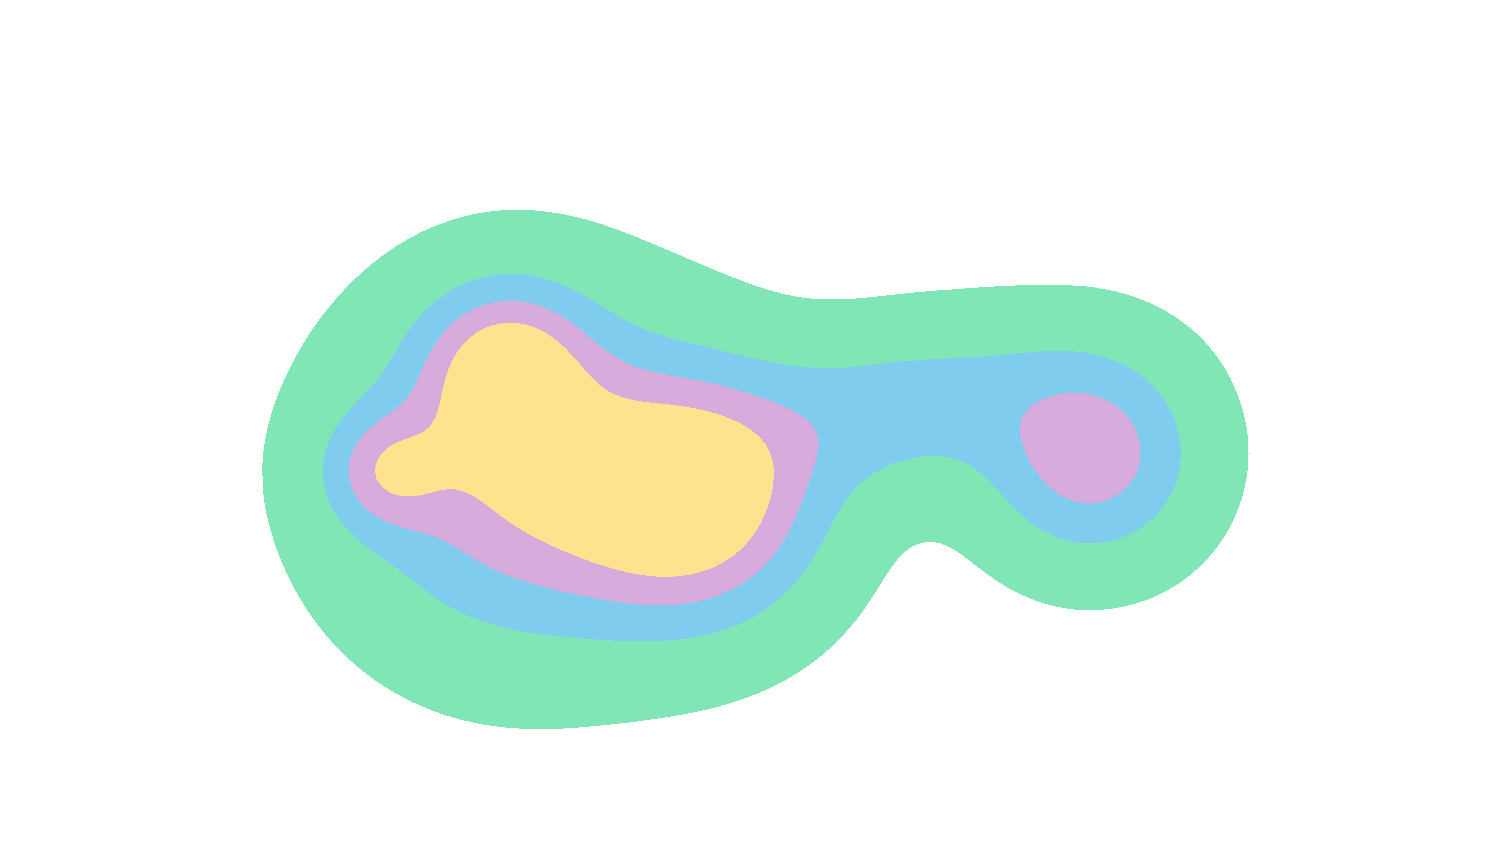
\includegraphics[trim=250 0 50 100, clip, width=0.35\textwidth]{figures/surf-top.png}
  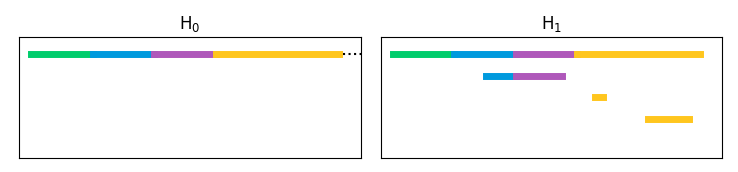
\includegraphics[width=0.8\textwidth]{figures/scalar_barcode_true.png}
  \caption{A scalar field on a 2D domain and its persistence barcode.}
\end{figure}

\paragraph*{Contribution}

We will re-cast the TCC as a way to verify that the persistent homology of a scalar field can be \emph{partially} approximated by a given sample.
Specifically, we will relate the persistent homology of a function relative to a \emph{static} sublevel set to a \emph{truncation} of the full diagram.
That is, beyond a certain point the full diagram remains unchanged, allowing for possible reconstruction.
% While the approximation of a function's persistent homology is well studied in general~\cite{chazal08towards}, the presence of incomplete data can severely impact the quality of the approximation.
% That is, due to the nature of homology as a measure of global structure, the \emph{restricted} diagram resulting from removing un-verified data fills in missing global structure with potentially spurious features.
This is in comparison with the \emph{restricted} diagram obtained by simply ignoring part of the domain.
% Due to the nature of homology as a measure of global structure that the restricted diagram may attempt to fill in, resulting in spurious features.
We therefore present relative persistent homology as an alternative to restriction in a way that extends the TCC to the analysis of scalar fields.
 % the presence of incomplete data can severely impact the quality of an approximation.
% This is primarily due to the nature of homology as a measure of global structure.
% That is, beyond a certain point the full diagram remains unchanged, allowing for possible reconstruction.
% While the obvious solution is to simply remove the un-verified data, the resulting \emph{restricted} diagram fills in missing global structure with potentially spurious features.
% Indeed, it can be shown that the truncated diagram is captured by the restriction in a specific way~\cite{cohen09extending, desilva11duality}.
% We therefore provide experimental evidence that compares the approximation of the restricted function directly provides a worse interleaving with the corresponding subset of the \emph{full} diagram.

Section~\ref{sec:summary} establishes notation and provides an overview of our main results in Sections~\ref{sec:tcc} and~\ref{sec:middle}.
In Section~\ref{sec:truncations} we introduce an interpretation of the relative diagram as a truncation of the full diagram that is motivated by a number of experiments in Section~\ref{sec:experiments}.% in terms of the sublevel set filtration as a \emph{truncation}.
